\chapter{Stato dell'arte} %\label{1cap:spinta_laterale}
% [titolo ridotto se non ci dovesse stare] {titolo completo}
%
Questo capitolo illustra lo stato dell’arte e i lavori presenti in letteratura sugli aspetti di ricerca trattati nel nostro studio.

Dagli articoli presenti in letteratura è emerso che l’uso dei chatbot si è evoluto rapidamente in numerosi campi negli ultimi anni, tra cui marketing, sistemi di supporto, istruzione, assistenza sanitaria, beni culturali e intrattenimento. I chatbot sono anche conosciuti come robot intelligenti, agenti interattivi, assistenti digitali o entità di conversazione artificiali.  Essi possono imitare la conversazione umana e intrattenere gli utenti, sono anche utili in applicazioni riguardanti istruzione, reperimento di informazioni, affari ed e-commerce. Sono diventati così popolari perché ci sono molto vantaggi sia per utenti che per sviluppatori. \cite{adamopoulou2020overview}

L’interesse per lo sviluppo dei chatbot è in aumento e con esso è cresciuto anche il numero di studi sperimentali condotti sull’usabilità dei chatbot. 
In generale, i risultati sperimentali hanno rivelato che i chatbot hanno diversi vantaggi, forniscono una risposta in tempo reale e migliorano la facilità d’uso, ma anche diverse carenze, ad esempio, l’elaborazione del linguaggio naturale, è considerata la debolezza più bisognosa di miglioramento.\cite{9687577}

A partire dal concetto di “chatbot” è stata sviluppata una loro evoluzione, orientata all’aiuto nello sviluppo del software negli Integrates Development Environments (IDEs). Una caratteristica fondamentale all’interno di questi ultimi è l’aiuto che forniscono nel completamento del codice. 
Sviluppare software di alta qualità riducendo il time-to-market è uno degli obiettivi più ambiziosi all’interno dell’industria di sviluppo software. 

Per ridurre il time-to-market è necessario incrementare la produttività degli sviluppatori riducendo il tempo di apprendimento di un linguaggio e migliorare il codice scritto prevenendo potenziali bug in fase di scrittura. In risposta a queste necessità, i ricercatori hanno proposto dei sistemi per l’ingegnerizzazione del software inseguendo il sogno di una vita, ovvero la generazione automatica del codice sorgente. \cite{wen2021siri}

Una delle estensioni per IDE più interessanti è Github Copilot per Visual Studio Code, esso fornisce allo sviluppatore dei suggerimenti basati sulla descrizione di un problema da risolvere e sul codice esistente. Basato su un modello per linguaggi in larga scala, Codex, un ulteriore sviluppo di GPT-3 \cite{brown2020language}, il cui training è stato effettuato su codice sorgente, GitHub Copilot è molto di più che un semplice aiuto nel completamento del codice dato dall'IDE, in quanto non solo può suggerire il completamento del codice, ma anche un un'intera funzione basandosi sulle richieste dello sviluppatore scritte in linguaggio naturale. \cite{sobania2021choose}
\bigbreak
\begin{python}
'''
Function to unizip a file
'''
\end{python}
\begin{lstlisting}[frame=none,caption={Commento scritto dallo sviluppatore},captionpos=b,label=copilotinput]
\end{lstlisting}
\begin{python}
'''
Function to unizip a file
'''
import zipfile
import os
import sys
import shutil

def unzip(filename):
    zip_ref = zipfile.ZipFile(filename, 'r')
    zip_ref.extractall('.')
    zip_ref.close()
\end{python}
\begin{lstlisting}[frame=none,caption={Codice generato da GitHub Copilot},captionpos=b,label=copilotoutput]
\end{lstlisting}
\newpage
\section{Anatomia di un Conversational Agent}
Un'architettura di riferimento per un conversational agent è quella che vede l'utilizzo dei seguenti componenti:
\begin{itemize}
    \item 1) \textbf{Riconoscimento Vocale}. Se l'applicazione fornisce un'interfaccia vocale con la quale l'utilizzatore può fornire dei comandi, è necessario che il conversational agent sia in grado di trasformare, tramite l'utilizzo di un apposito componente, il parlato in input in un comando da fornire al bot e la risposta in output in una clip audio da fornire al richiedente.\cite{srivastava2019reference}
    
    \item 2) \textbf{Intents e Parametri}. Gli intents sono delle classi di input predefinite che vengono assegnate ai bot da parte degli sviluppatori. ovvero quello che l'applicativo si aspetta di ricevere come comando. I parametri invece, sono degli attributi ricavati dalla lettura degli input e servono ad effettuare un'azione o dare una risposta, qualche esempio nella tabella sottostante:
    \begin{table}[h]
    \centering
    \begin{tabular}{|lll|} 
    \hline
    \textbf{Input}              & \textbf{Intent}               &     \textbf{Parametri}     \\ 
    \hline
    Voglio prenotare un albergo & Prenotazione                  &     \textit{Null}          \\ 
    \hline
    Voglio prenotare un treno~  & \multirow{3}{*}{Prenotazione} &     Partenza: Milano       \\
    da Milano a Salerno~        &                               &     Destinazione:Salerno~  \\
    il 29/02/2023               &                               & Data:     2023-02-29       \\ 
    \hline
    Siete aperti a cena?~       & Richiesta~                    &     Dettaglio: Orario      \\ 
    \hline
    Prodotto impeccabile!~      & Feedback~                     &     Sentimento: Positivo   \\
    \hline
    \end{tabular}
    \end{table}
    
    La classificazione degli intent è gestita da un componente chiamato \textit{Intent Classifiers}. Invece estrarre i parametri è un lavoro fatto dal componente detto \textit{Parameters Extractor}. 
    Ovviamente parametri e intents potrebbero non includere tutte le possibili combinazioni, se non si riuscisse a classificare l'intent, ne esiste uno di "default". 
    
    La maggior parte delle soluzioni in commercio sono già predisposte tramite un modello \textit{blackbox}, è lo sviluppatore a fornire intent, parametri e frasi di esempio grazie ai quali il modello sarà addestrato.\pagebreak
    
    \item 3) \textbf{Risponditore}: Come nelle conversazioni tra umani, il risponditore si occupa di generare risposte dagli input ricevuti. Ovviamente nel caso in cui l'input non sia riconoscibile la risposta generata sarà quella in cui verrà chiesto all'utente di riformulare la richiesta. La risposta generata può essere statica o dinamica. 
    
    Una risposta statica può essere un tipico saluto di benvenuto, (es. \textit{"Bentornato Mario"}) mentre quella dinamica dovrà essere generata in base ad input e dettagli esterni (es. \textit{"La consegna verrà effettuata entro le ore 22:00"}). 
    
    Una classe di risposte semi-dinamiche sono le domande che il risponditore fa all'utente a seguito di una richiesta (es. \textit{"A che ora vuoi prenotare il tavolo stasera?"}). Il risponditore può inoltre comunicare con altri componenti del sistema per decidere la risposta da dare all'utente.
    
    \item 4) \textbf{Controllore del Flusso}: Si occupa di mantenere lo stato della conversazione per decidere qual è la prossima azione da compiere. Per esempio può inviare la richiesta di prenotazione della camera se la domanda precedente era \textit{"Vuoi confermare la prenotazione?"} e la risposta dell'utente è \textit{"Si"} o semplicemente decidere di richiedere all'utente nuovamente delle informazioni sulla prenotazione riportando lo stato corrente a qualche domanda precedente. Per fare questo utilizza i \textit{Context Objects} ognuno dei quali mantiene lo stato ad un determinato istante nel tempo.
    
    \item 5) \textbf{Azione ed Eseguibili}: il lavoro dei componenti è quello di fornire un interfaccia tramite linguaggio naturale all'utente, per interagire con l'applicazione. Le funzionalità principali che l'applicazione fornisce sono disaccoppiate dai componenti. Queste azioni servono per creare un ponte tra le funzionalità principali dell'applicazione e i componenti. E' il controllore del flusso che chiama un determinato eseguibile basandosi sugli eventi, un evento rappresenta una specifica condizione che accade durante una conversazione con l'utente. Per esempio, se l'intent classifier si accorge che l'utente ha intenzione di prenotare un treno ed il parameter extractor ha estratto tutti i dettagli necessari, il controllore del flusso può eseguire l'azione "l'utente ha richiesto di prenotare il treno".\cite{srivastava2019reference}
    \end{itemize}\pagebreak
    
\section{Utilizzo di conversational agent nello smart development}
Gli sviluppatori che si trovano a risolvere un problema nello sviluppo moderno, raramente si trovano a dover riscrivere il codice da zero.

Piattaforme come Github e StackOverflow, forniscono milioni di esempi di codice per quasi tutte le attività di programmazione immaginabili. L'apprendimento automatico potrebbe rendere il lavoro ancora più semplice.

La sfida per la ricerca è ora trasferire i  successi dei modelli linguistici nell'elaborazione del linguaggio naturale ai linguaggi di programmazione con la loro semantica ancor più precisa. Il desiderio di programmi che scrivono programmi è vecchio quanto  l' informatica. \cite{finkbeiner2021kunstliche} 

Già nel 1957 Alonzo Church, uno dei fondatori della disciplina, all'epoca ancora giovane, formulò la sfida: \textit{"è possibile tradurre automaticamente un'attività da compiere in un programma per computer, cioè tramite un algoritmo, in modo che il programma risolva correttamente l'attività per ogni possibile input?"}. 

Oggi a più di 60 anni di distanza la risposta sembra a portata di mano grazie a modelli di linguaggio come GPT-3 (Generative Pre-trained Transformer)\cite{chintala_2020}\bigbreak
\begin{python}
def compute_total_price(self, palindrome_discount=0.2):
    """
    Compute the total price.
    Apply a discount to items whose names are palindromes
    """
    total_price = 0
    for item in self.items:
       if is_palindrome(item.name):
          total_price += item.price * (1 - palindrome_discount)
       else:
          total_price += item.price
    return total_price
    
\end{python}
\textit{GPT-3 genera codice. Un compilatore da linguaggio naturale, commento in rosso, a codice} \cite{crivello_2020}

\newpage
\section{I Dataset}
In questo paragrafo è descritto l'utilizzo dei dataset all'interno dei linguaggi di modello, in particolare esamineremo The Pile, HumanEval e APPS questi ultimi due sono Dataset utilizzati per il test dei modelli di program synthesis permettendone di valutarne il grado di risoluzione in problemi di programmazione.
\subsection{The Pile}
The Pile e' un dataset basato su testi in inglese da 825 GiB destinato al training di modelli linguistici su larga scala, esso è stato creato sulla base di 22 dataset preesistenti, che comprendono sia dataset consolidati per l'elaborazione del linguaggio naturale sia alcuni di nuova introduzione.

Il dataset viene creato da varie origini di dati, inclusi i libri; repository GitHub; pagine web; chat; articoli di medicina, fisica, matematica, informatica e filosofia. In particolare, utilizza le seguenti fonti: Pile-CC, PubMed Central, ArXiv, GitHub, FreeLaw Project, Stack Exchange, US Patent and Trademark Office, PubMed, Ubuntu, IRC, HackerNews, YouTube, PhilPapers, Books3, Project Gutenberg ( PG-19), OpenSubtitles, Wikipedia in inglese, DM Mathematics, EuroParl, Enron Emails corpus e NIH ExPorter. Include anche OpenWebText2 e BookCorpus2, che sono rispettivamente estensioni dei dataset originali OpenWebText e BookCorpus. La diversità delle fonti di dati può migliorare le conoscenze generali tra domini e di conseguenza migliorare le capacità di generalizzazione a valle.

Oltre alla sua utilità per l'addestramento di modelli linguistici di grandi dimensioni, The Pile può anche servire come benchmark.

Recenti studi hanno dimostrato che, soprattutto per modelli di grandi dimensioni, la diversità delle fonti di dati migliora la conoscenza trasversale del modello e la capacità di generalizzazione. Non solo i modelli addestrati su Pile mostrano miglioramenti nei benchmark tradizionali di modellazione linguistica, ma anche miglioramenti significativi in Pile BPB. 
Pile BPB (Bits per Bits) è un robusto benchmark della capacità di modellazione testuale generale e trasversale per i modelli linguistici di grandi dimensioni che misura la conoscenza del mondo e della capacità di ragionamento. \cite{pile}

La sfida principale con questo dataset è l'enorme dimensione; con i suoi 825 GiB di testo, che si traducono in 4.2 TiB di dati preelaborati e compressi. Si può da subito intuire che il training di un modello con questo dataset su una singola istanza richiederà molto tempo e non è molto pratico.
\newpage
\subsection{HumanEval}
HumanEval è un dataset di 164 problemi di programmazione scritti a mano, ognuno dei quali include una firma di funzione, documentazione, corpo e alcuni unit test. I problemi di programmazione del dataset valutano la comprensione della lingua, il ragionamento, gli algoritmi e alcuni problemi di matematica semplice. \cite{https://doi.org/10.48550/arxiv.2107.03374}
E' stato creato ed utilizzato per testare alcuni modelli di linguaggio adatti al completamento del codice come Codex e GPT-Neo.
\subsection{APPS}
APPS (Automated Programming Progress Standard) è costituito da problemi raccolti da diversi siti web, come Codeforces, Kattis e altri ed è utilizzato principalmente per effettuare benchmark. Il benchmark APPS cerca di rispecchiare il modo in cui vengono valutati i programmatori umani, ponendo problemi di codifica in un linguaggio naturale e utilizzando casi di test per valutare la correttezza della soluzione. I problemi hanno un grado di difficoltà che va da un livello base a quello di competizione Hackathon e misurano la capacità di codifica e di risoluzione dei problemi. (Figura \ref{fig_apps})

Consiste in un totale di 10.000 problemi di codifica, con 131.777 casi di test per la verifica delle soluzioni e 232.421 soluzioni, scritte a mano. La lunghezza media di un problema è di 293,2 parole, quindi spesso sono anche complicati. I dati sono suddivisi in training-set e test-set, con 5.000 problemi ciascuno. Ogni test-case è progettato in modo specifico per il problema corrispondente, consentendo di valutare rigorosamente la funzionalità del programma.\cite{DBLP:journals/corr/abs-2105-09938}
\begin{figure}[h!]
\centerline{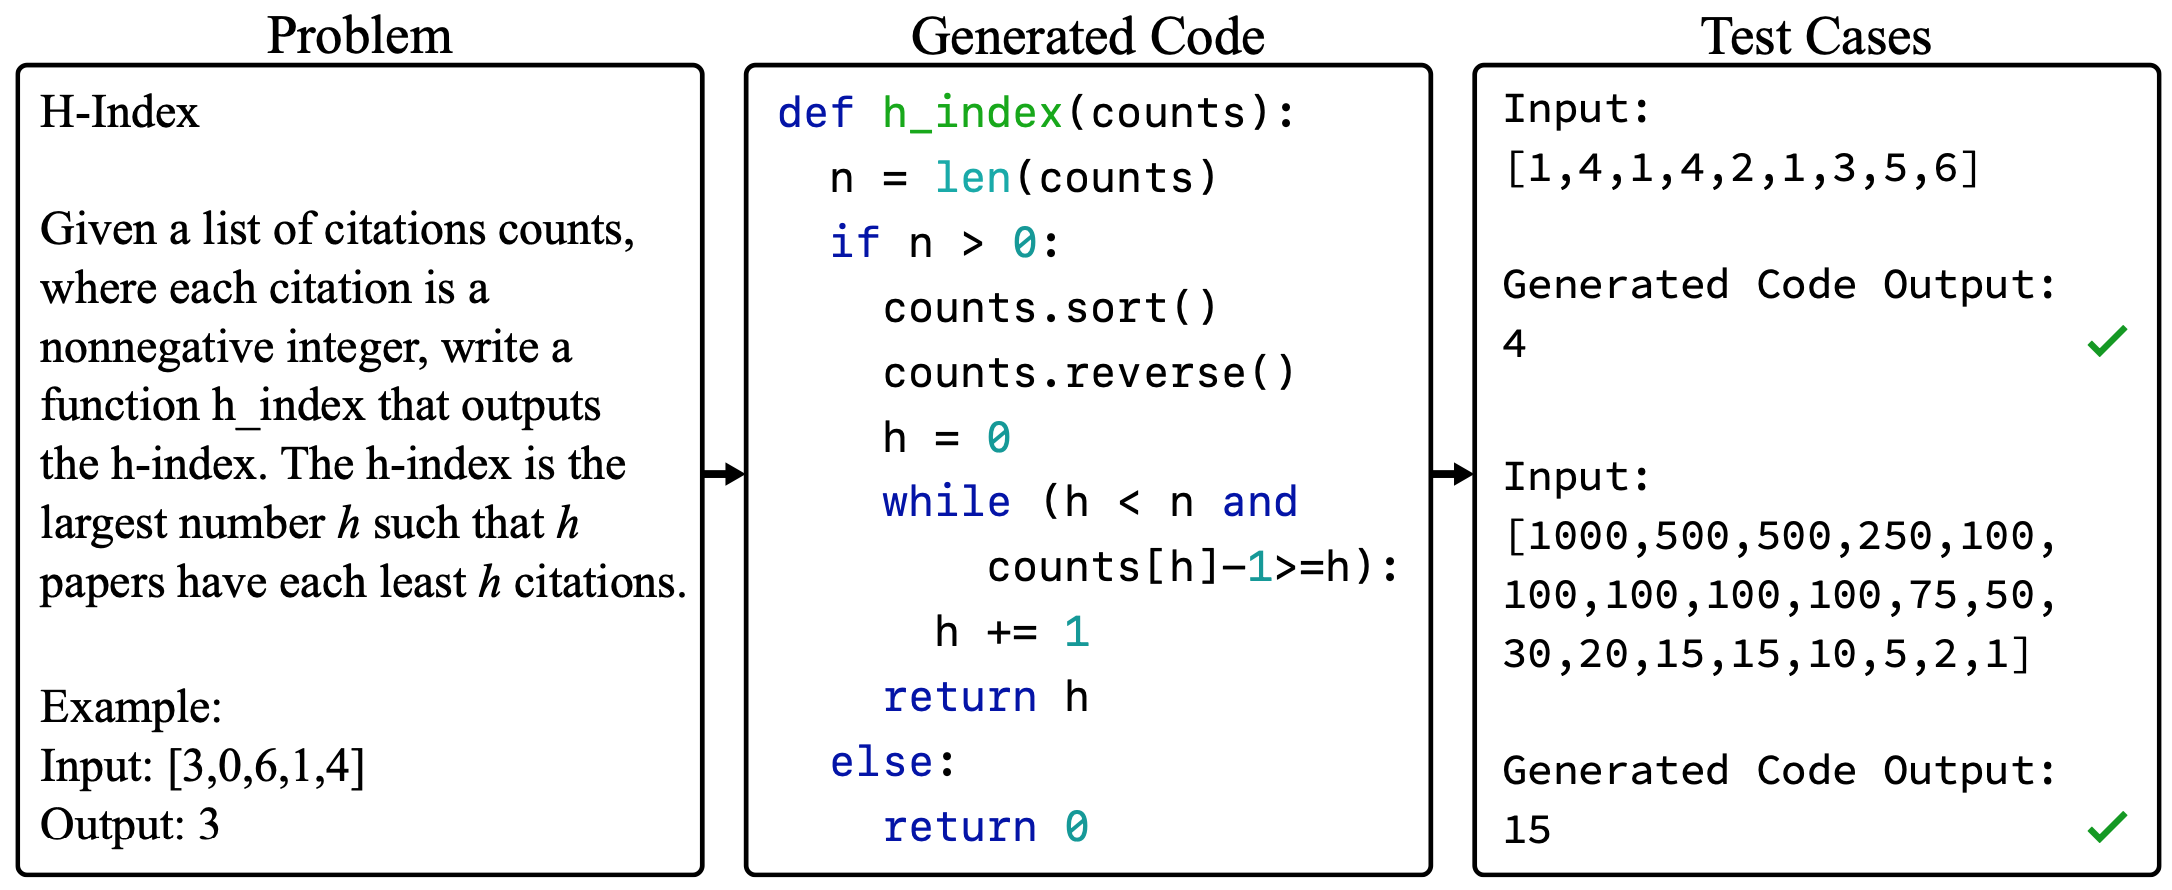
\includegraphics[scale=.40]{immagini/apps_example.png}}
\caption{Esempio di un problema in APPS (sinistra) insieme ad uno dei possibili codici generati (centro) e due esempi dei test case utilizzati per valutare il codice (destra)}
\label{fig_apps}
\end{figure}
\newpage

\section{Modelli di ML per generazione di codice}
In questo paragrafo daremo uno sguardo a quelli che sono i modelli NLP per la generazione del codice esistenti al momento della scrittura di questo documento.
\subsection{GPT-2}
GPT-2 è un modello linguistico basato su trasformatore di apprendimento profondo non supervisionato creato da OpenAI nel febbraio 2019 con l'unico scopo di prevedere le parole successive in una frase. GPT-2 è l'acronimo di "Generative Pretrained Transformer 2". 

Il modello è open source ed è addestrato su oltre 1,5 miliardi di parametri per generare la successiva sequenza di testo per una data frase. Grazie alla diversità del dataset utilizzato nel processo di addestramento, possiamo ottenere un'adeguata generazione di testo per il testo da una varietà di domini. GPT-2 è 10 volte i parametri e 10 volte i dati del suo predecessore GPT.

Le attività linguistiche come la lettura, il riepilogo e la traduzione possono essere apprese da GPT-2 dal testo grezzo senza utilizzare i dati di addestramento specifici del dominio.
Ci sono limitazioni che devono essere considerate quando si ha a che fare con la generazione del linguaggio naturale. I limiti includono testo ripetitivo, incomprensione di argomenti altamente tecnici e specializzati e incomprensione di frasi contestuali.

La lingua e la linguistica sono un dominio complesso e vasto che in genere richiede a un essere umano di sottoporsi ad anni di formazione ed esposizione per comprendere non solo il significato delle parole ma anche come formare frasi e dare risposte che siano contestualmente significative e per usare uno slang appropriato. Questa è anche un'opportunità per creare modelli personalizzati e scalabili per diversi domini. Un esempio fornito da OpenAI è addestrare GPT-2 utilizzando il dataset di Amazon Reviews per insegnare al modello a scrivere recensioni condizionate da cose come la valutazione a stelle e la categoria.

\subsection{GPT-3}
GPT-3 è un modello di linguaggio autoregressivo con 175 miliardi di parametri, 10 volte in più di ogni altro modello di linguaggio sparso. Ottiene risultati grandiosi su parecchi dataset NLP, incluse traduzioni e domande-risposte\cite{brown2020language}
I linguaggi NLP sono passati da imparare rappresentazioni di problemi e architetture legate in modo specifico ai compiti da eseguire, all'utilizzare training e architetture incuranti del compito da portare a termine. Questo salto ha portato a un progresso sostanziale in molte sfide, come tra le molte, quella di comprendere quanto letto, rispondere a domande o compiti basati sull'implicazione testuale.
Tra i vari tipi di approcci utilizzati da GPT-3 per imparare dal contesto sono stati utilizzati i seguenti:
\begin{itemize}
\item {\textbf{Fine-Tuning (FT)}} - Aggiorna i pesi di un modello pre-addestrato effettuando il training su migliaia di label supervisionate specifiche per il compito. Il principale vantaggio del fine-tuning è rappresentato da prestazioni elevate su parecchi benchmark. Gli svantaggi sono la necessità di un nuovo dataset di grandi dimensioni per ogni compito e la scarsa generalizzazione\cite{https://doi.org/10.48550/arxiv.1902.01007}
Few-Shot (FS) - Al modello vengono fornite alcune dimostrazioni del compito, ma non vengono aggiornati i pesi. Few-shot funziona dando {\textit{K}} esempi di contesto e altrettanti di completamento. Il vantaggio principale è la notevole riduzione della necessità di dati specifici. Lo svantaggio è che i risultati sono peggiori dei modelli con regolazione. fine.\cite{brown2020language}
\item {\textbf{One-Shot (1S)}} - Simile ad FS ma con \textit{K} = 1.
\item {\textbf{Zero-Shot (0S)}} - Simile ad FS ma con una descrizione in linguaggio naturale del compito invece che di esempi.
\cite{brown2020language}
\begin{table}[h!]
\centering

\end{table}
\begin{table}[h!]
    \centering
     \begin{tabular}{||c c c c c||} 
     \hline
     & LAMBADA & LAMBADA & StoryCloze & HellaSwag \\ [0.5ex] 
     Setting & (acc) & (ppl) & (acc) & (acc) \\ [0.5ex] 
     \hline\hline
     GPT-3 Zero-Shot & 76.2 & 3.00 & 83.2 & 78.9 \\ 
     GPT-3 One-Shot & 72.5 & 3.35 & 84.7 & 78.1 \\
     GPT-3 Few-Shot & 86.4 & 1.92 & 87.7 & 79.3 \\ [1ex] 
     \hline
     \end{tabular}
    \caption{Prestazioni di GPT-3 con i vari approcci elencati sopra\cite{brown2020language}}
    \label{tab:table1}
\end{table}
\end{itemize}
Il successo del consolidato strumento di completamento del codice Tabnine dà un'idea del potenziale di questo approccio. \cite{finkbeiner2021kunstliche}
\subsection{Codex}
Codex è un modello di linguaggio creato a partire da GPT sul quale è stato effettuato fine-tuning mediante codice pubblicamente disponibile su GitHub.
Il primo tentativo nella creazione di Codex è stato quello di effettuare un fine-tuning sulla famiglia dei modelli di GPT-3, non sono stati però rilevati miglioramenti pertanto successivamente è stato utilizzato GPT come modello di partenza. A differenza di GPT, Codex sul dataset HumanEval ha mostrato risultati non indifferenti. Infatti riesce a risolvere la maggior parte dei problemi presenti nel Dataset.
\begin{figure}[h!]
\centerline{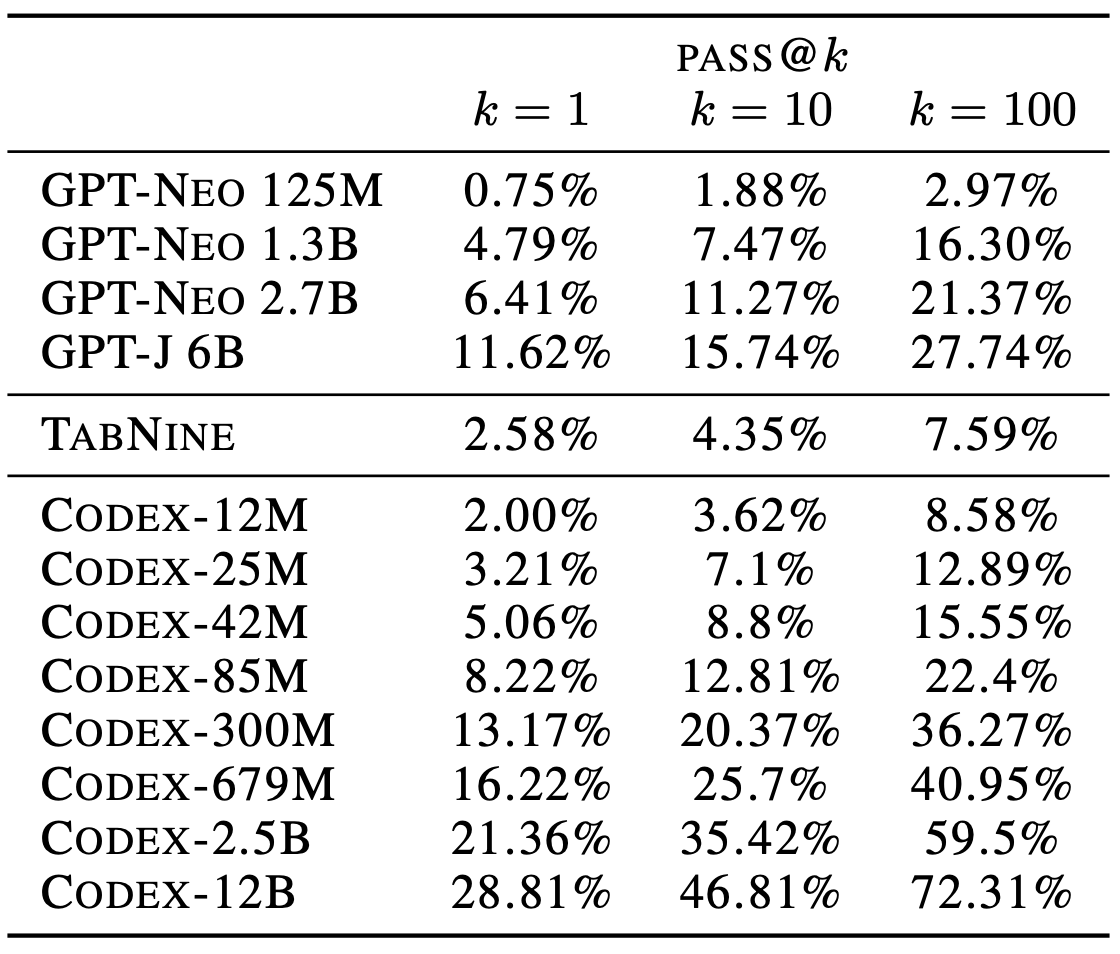
\includegraphics[scale=.40]{immagini/humaneval_results.png}}
\caption{Risultati di alcuni modelli su HumanEval}
\label{fig_humaneval}
\end{figure}

\subsection{InCoder} \label{sssec:num1}
InCoder è un modello unificato per la program synthesis. 
È addestrato a generare file di codice da un ampio corpus di codice, in cui alcune regioni sono state mascherate in modo casuale e spostate alla fine di ogni file.
Impara a riempire sostituendo in modo casuale gli intervalli di codice con un token sentinella e spostandoli alla fine della sequenza.(Figura \ref{fig1_incoder})
\begin{figure}[h]
\centerline{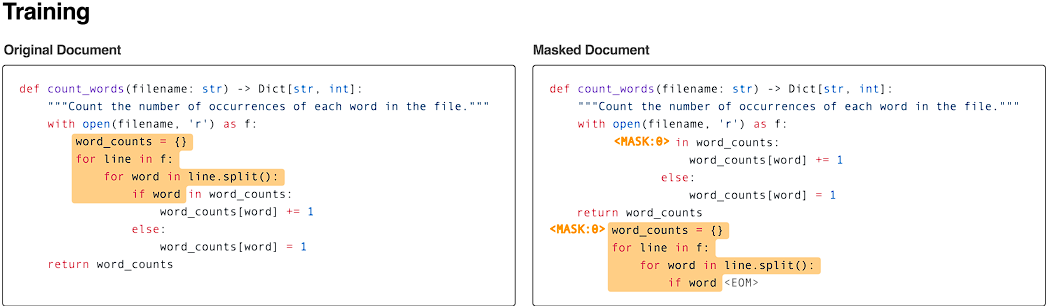
\includegraphics[scale=.70]{immagini/incoder_fig1.png}}
\caption{Esempio di mascheramento di InCoder}
\label{fig1_incoder}
\end{figure}
Il modello viene addestrato a prevedere tutti i token della sequenza completa. Durante l'inferenza, può modificare il codice sostituendo gli intervalli con i token sentinella, chiedendo al modello la nuova sequenza e facendogli generare nuovi token per sostituire gli intervalli mascherati. (Figura \ref{fig2_incoder})
\begin{figure}[h!]
\centerline{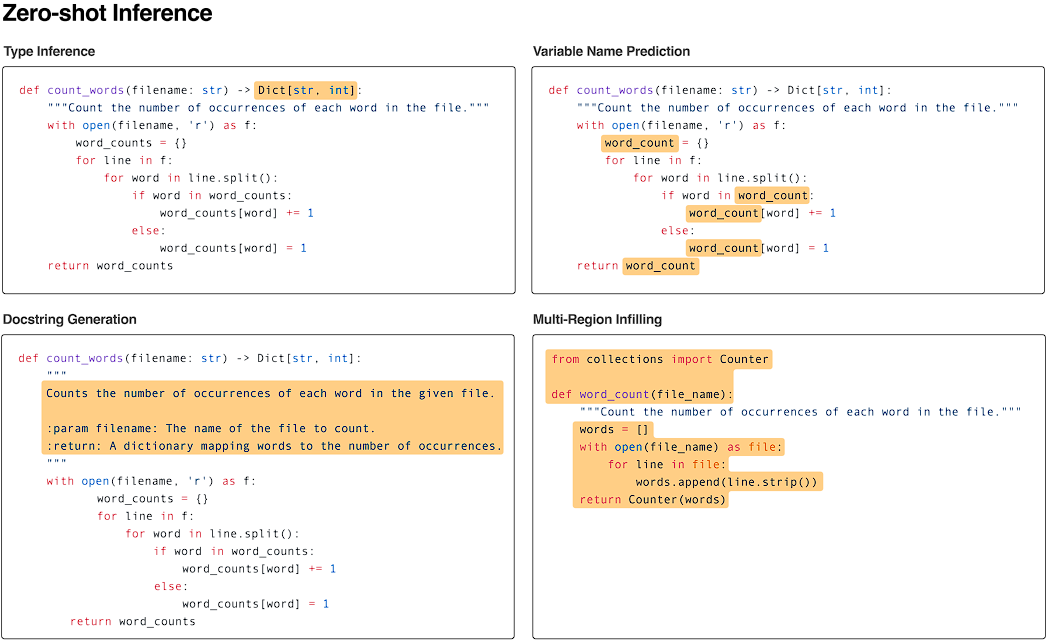
\includegraphics[scale=.70]{immagini/incoder_fig2.png}}
\caption{Esempio di generazione del codice di InCoder}
\label{fig2_incoder}
\end{figure}
I dati su cui è stato effettuato il training di InCoder sono stati presi da codice pubblico open-source da GitHub e GitLab, domande e risposte da StackOverflow con un focus particolare sul linguaggio Python.

\section{Impatto sociale}
Open AI ha descritto accuratamente quale potrebbe essere l'impatto di un modello di linguaggio addestrato su codice esistente presente all'interno dei dataset, come quelli di cui abbiamo parlato nel paragrafo precedente.
\begin{itemize}
    \item {\textbf{Eccessiva Fiducia nel Modello}}: un modello linguistico addestrato su grandi insiemi di dati  con il compito di autogenerare codice può generare soluzioni plausibili che possono sembrare corrette, ma non necessariamente lo sono. La mancata valutazione del codice generato può avere conseguenze negative, come l'introduzione di bug o di vulnerabilità di sicurezza. Pertanto, è importante che gli utenti siano consapevoli dei limiti e delle potenziali conseguenze negative dell'utilizzo di un modello linguistico addestrato su questo set di dati. \cite{https://doi.org/10.48550/arxiv.2107.03374}
    \item {\textbf{Impatto economico e sul mercato del lavoro}}: i grandi modelli linguistici addestrati su grandi insiemi di codice come GPT-3, in grado di generare codice di alta qualità, hanno il potenziale di automatizzare parte del processo di sviluppo del software. Ciò potrebbe avere un impatto negativo sugli sviluppatori di software. Tuttavia, come discusso nel documento, e come mostrato nel Rapporto di sintesi sugli sviluppatori di software di O*NET OnLine, gli sviluppatori non scrivono solo software.\cite{https://doi.org/10.48550/arxiv.2107.03374}
    \item {\textbf{Implicazioni per la sicurezza}}: non è stato effettuato alcun filtro o controllo delle vulnerabilità o del codice difettoso. Ciò significa che il dataset può contenere codice che può essere dannoso o contenere vulnerabilità. Pertanto, qualsiasi modello addestrato su questo set di dati può generare codice vulnerabile, con presenza di bug o dannoso. Questo potrebbe portare a un software che potrebbe funzionare in modo improprio e causare gravi conseguenze a seconda del software. Inoltre, un modello addestrato su questo set di dati potrebbe essere utilizzato per generare di proposito codice dannoso al fine di eseguire ransomware o altri attacchi simili.\cite{https://doi.org/10.48550/arxiv.2107.03374}
    \item{\textbf{Implicazioni legali}}: non è stato eseguito alcun filtraggio sul codice con licenza. Ciò significa che il dataset può contenere codice con licenza restrittiva. Come discusso nel documento, i repository Github pubblici possono rientrare nel "fair use". Tuttavia, in passato sono stati registrati pochi casi di utilizzo di codice disponibile su licenza. Pertanto, qualsiasi modello addestrato su questo set di dati potrebbe essere tenuto a rispettare i termini di licenza in linea con il software su cui è stato addestrato, come ad esempio la GPL-3.0, motivo per cui abbiamo volutamente messo questo set di dati sotto la licenza GPL-3.0. Non sono chiare le conseguenze legali dell'uso di un modello linguistico addestrato su questo dataset.\cite{https://doi.org/10.48550/arxiv.2107.03374}
\end{itemize}
\section{Cosine Similarity}
La cosine similarity è una metrica ampiamente implementata nell’information retrieval e negli studi correlati. Questa metrica modella un documento di testo come un vettore di termini. In base a questo modello, la somiglianza tra due documenti può essere ricavata calcolando il coseno tra i vettori di termini dei due documenti.

L’implementazione di questa metrica può essere applicata a due documenti che siano essi frasi, paragrafi o documenti interi. I valori di similarità tra la query e i documenti sono ordinati dal più alto al più basso, una similarità elevata tra il vettore del documento e quello della query indica una maggiore pertinenza tra i due. 

La cosine similarity per valutare la somiglianza tra il documento e la query dell’utente dovrebbe adattarsi al significato della parola; tuttavia, ancora non si è in grado di gestire perfettamente il significato semantico del testo.

L’implementazione della cosine similarity, a volte, produce risultati inaffidabili dal punto di vista sintattico. Per risolvere questo problema sono stati condotti studi sulla misurazione semantica o sulla somiglianza semantica tra le parole. Il metodo più comune utilizza un database lessicale come rete semantica cioè WordNet. 

Attraverso l’esplorazione di questo database si può ricavare la somiglianza tra due concetti, basandosi sul giudizio umano e non solo sulla cosine similarity. WordNet si propone di modellare la conoscenza lessicale di una madrelingua inglese. L’unità più piccola di WordNet è un gruppo logico chiamato synset, che rappresenta il senso di una parola. I synset hanno relazioni semantiche tra loro.
Un documento può essere descritto in forma vettoriale come:
\begin{center}
\scaleto{\vec{d}=(W_{d0},W_{d1},...,W_{dk})}{15pt}
\end{center}
La query può essere descritta in forma vettoriale:
\begin{center}
\scaleto{\vec{q}=(W_{q0},W_{q1},...,W_{qk})}{15pt}
\end{center}
Dove $W_{di}$  e  $W_{qi}$ $(0 \leq i \leq k)$ sono float che indicano la frequenza di ogni termine all’interno di un documento, mentre la dimensione di ogni vettore corrisponde a un termine disponibile nel documento.
In base alla cosine similarity, la similarità tra due vettori può essere definita come:
\begin{center}
\scaleto{Sim(\vec{q},\vec{d})=\frac{\vec{q}\cdot \vec{d}}{\left |\vec{q} \right|\left | \vec{d} \right |}=\frac{\sum_{k=1}^{t}W_{qk}\times W_{dk}}{\sqrt{\sum_{k=1}^{t}\left ( W_{qk} \right )^{2}\cdot \sqrt{\sum_{k=1}^{t}\left ( W_{dk} \right )^{2}}}}}{40pt}
\end{center}
La Cosine similarity può essere applicata solo a vettori della stessa dimensione altrimenti otterremmo un valore di similarità bassa, quando il valore di similarità è troppo basso è diverso dal giudizio umano. Attualmente sono in corso studi al fine di migliorare la similarità del coseno tra due vettori di termini basandosi sul giudizio umano.

Nello scenario sopra descritto, la somiglianza del coseno tendente a \texttt{1} implicherebbe che i due documenti sono esattamente simili mentre una somiglianza del coseno tendente a \texttt{0} porterebbe alla conclusione che non ci sono somiglianze tra i due documenti. Vediamo un esempio:

\begin{center}
\texttt{Frase 1: Il deep learning può essere difficile}

\texttt{Frase 2: Il deep learning può essere semplice}
\end{center}
Per prima cosa otteniamo una rappresentazione vettorializzata dei testi, per farlo, si analizzano le singole parole distinte con significato all'interno della frase, eliminando da esse congiunzioni e articoli:
\begin{table}[h]
    \centering
    \begin{tabular}{|c|c|c|c|c|c|c}
    \hline
         Deep & Learning & può & essere & difficile & semplice  \\
         \hline
    \end{tabular}
    \label{tab:tabvettorecosinesimilarity}
\end{table}

Dopodiché per ogni frase si va ad assegnare alla posizione \texttt{i-esima} del vettore un valore \texttt{1} oppure \texttt{0} rispettivamente se la parola è presente all'interno della frase o meno. Chiamiamo i due documenti A e B, otteniamo quindi la seguente rappresentazione vettoriale:

\begin{table}[h]
\centering
\begin{tabular}{|c|c|c|c|c|c|c|}
\hline
        & Deep  & Learning  & Può       & Essere    & Difficile & Semplice  \\ \hline
A & 1     & 1         & 1         & 1         & 1         & 0         \\ \hline
B & 1     & 1         & 1         & 1         & 0         & 1         \\ \hline
\end{tabular}
\end{table}

Utilizzando questi vettori e la formula vista in precedenza possiamo procedere con il calcolo della consine similarity.

\begin{center}
\scaleto{Sim(\vec{A},\vec{B})=\frac{\vec{A}\cdot \vec{B}}{\left |\vec{A} \right|\left | \vec{B} \right |}}{38pt}
\end{center}
Andiamo dapprima a calcolare il prodotto scalare tra $\vec{A}$ e $\vec{B}$:
\begin{equation}
    \vec{A}\cdot \vec{B}=1\cdot1+1\cdot1+1\cdot1+1\cdot1+1\cdot0+0\cdot1=4
\end{equation}
Successivamente calcoliamo la norma dei due vettori:
\begin{equation}
    \left |\vec{A} \right|=\sqrt{1^2+1^2+1^2+1^2+0^2}=2.2360679775
\end{equation}
\begin{equation}
    \left |\vec{B} \right|=\sqrt{1^2+1^2+1^2+0^2+1^2}=2.2360679775
\end{equation}
Pertanto la cosine similarity sarà uguale a:
\begin{equation}
    \scaleto{Sim(\vec{A},\vec{B})=\frac{\vec{A}\cdot \vec{B}}{\left |\vec{A} \right|\left | \vec{B} \right |}=\frac{4}{2.2360679775*2.2360679775}\simeq0.8}{40pt}
\end{equation}
Ovvero da questo possiamo dedurre che abbiamo una somiglianza pari all'80\% tra le frasi estrapolate dai due documenti.